\documentclass[class=book, crop=false]{standalone}
\usepackage[subpreambles=true]{standalone}
\usepackage{import}
\usepackage[ruled,vlined]{algorithm2e}

\usepackage{amsmath}
\usepackage{amssymb}
\usepackage[margin=1.2in]{geometry}
\usepackage[sorting = none,
            doi = true  %lesedato for url-adresse
            ]{biblatex} %none gir bibliografi i sitert rekkefølge
\addbibresource{reference.bib}
\usepackage{csquotes}
\usepackage{pgfplots}
\pgfplotsset{compat=1.15}

\begin{document}
There are many ways of setting up the state space and reward function that can result in very different behaviour of the agent. This chapter will present results from certain formulation of the reinforcement environment.
\section{Formulation 1 - Free activation}
A reinforcement agent was trained with reward function that does not include cost of activation. This is not a realistic case, since households that offer flexibility should be compensated for altering their energy profile. This formulation serves to show how an agent would activate flexibility if there was no direct cost associated with altering the power consumption. However, the agent is penalised for changing the total daily energy demand in the power net. Note that it is not penalised for changing the daily consumption at individual loads as long as the total consumption in the network is preserved. The specific reward terms with weights are shown in table \ref{table:results:reward_formulation1}

\begin{table}[ht]
\centering
\caption{Reward terms and weights for formulation 1}
\label{table:results:reward_formulation1}
\begin{tabular}{l|ll}

Cost  & Weight & Comment
\\ 
\hline
Voltage &
1 &
Per-unit values
\\
Current &
$10^{-2}$ &
Percentage of max current 
\\
Activation &
0&
No activation cost
\\
Imbalance &
$10^{-4}$&
Units of energy imbalance is kWh
\\
\hline
\end{tabular}
\end{table}
The state space is constructed to be as small as possible. The state is represented by a 4 hour forecast for both solar irradiance and active power demand. The power demand is assumed equal at each flexible load, so there is not a individual power demand for each load. The total power imbalance for the whole power network is also included. Table \ref{table:results:state_formulation1} summarises the state space

\begin{table}[ht]
\centering
\caption{State used in formulation 1}
\label{table:results:state_formulation1}
\begin{tabular}{l|lll}

State space  & Size & Comment
\\ 
\hline
Solar forecast      &  4  &  4 hour solar forecast
\\ 

Demand forecast    &4 & One 4 hour forecast for all loads
\\ 
Imbalance state & 1  & Total energy imbalance for all loads
\\
\hline
\end{tabular}
\end{table}
The DDPG agent was trained for 100 000 time steps. A complete summary with all hyper-parameters used can be found in appendix ??. Figure \ref{fig:results:configuration1} visualises the actions of the trained agent throughout a day (24 hours) together with the solar irradiance. Because the solar power production in the system is very large, the safety margins for current and voltage are frequently violated. The desired behaviour of the agent is therefore to increase consumption in periods with high solar irradiance. This helps the system because the energy need not be transported out to the grid, but is consumed locally, close to production. Simply put, it is desired that the actions follow the curve of the solar irradiance. By inspecting figure \ref{fig:results:configuration1} it is clear that the agent  for several loads activate flexibility in times with much solar production. For instance, the plot \texttt{load = sun 10} in the bottom row clearly follows this pattern. The agent increases its power consumption during periods with high solar production, and reduces it later to ensure that the energy consumption is shifted, and not altered in absolute magnitude. The first plot in the top row \texttt{load = load 1} show some peculiar behaviour. Clearly, the actions do not follow the solar profile that day, but seem to be negative most of the day. This behaviour could be a result of how the reward function is defined in this configuration. The agent is penalised according to the total energy imbalance in the system, not at individual loads. As a result, if the energy imbalance is +10 MWh at one load and -10 MWh at another load, they perfectly cancel each other, and the agent is not penalised. From the agent's perspective, the system is in energy balance, although individual loads have a large absolute energy imbalance. This illustrates the problem with constructing state variable that accounts for the system as a whole, and not individual loads.  

\begin{figure}[ht]
    \center
    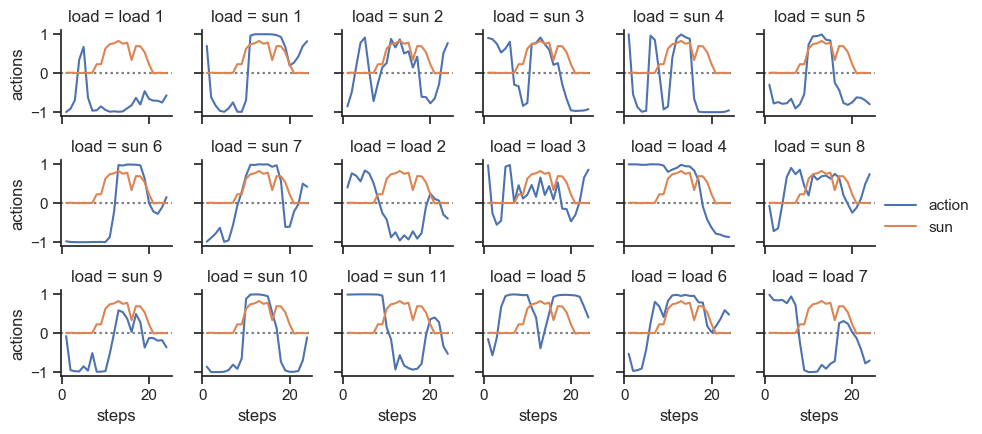
\includegraphics[height=8cm, width=15cm]{figures/configuration1.png}
    \caption[size = 9]{Activation of flexibility at the different flexible loads of the trained DDPG throughout a day. The orange line is the solar irradiance during the day, which is the same for all loads. The actions in blue is the activation of flexibility. Action = 1 means that the flexible load increases its power consumption with 10 \%, while action = -1 means that it decreases its power consumption with 10 \%}
    \label{fig:results:configuration1}
\end{figure}

\end{document}